
\chapter{Work}
\label{chap:work}
% **************************** Define Graphics Path **************************
\ifpdf
    \graphicspath{{Chapter3/Figs/Raster/}{Chapter3/Figs/PDF/}{Chapter3/Figs/}}
\else
    \graphicspath{{Chapter3/Figs/Vector/}{Chapter3/Figs/}}
\fi

The aim of this study was to capture the iterative elongation process
of even-chain saturated Fatty Acids. Fatty Acids are 
carboxylic acids with long hydrocarbon side groups
(Figure~\ref{fig:fas}) and they are usually characterised by the
number of carbons in these side-groups, for example a FA with a chain
of 6 carbons is usually denoted as $C_6$. The side-chains of FAs grow
by successive $C_2$ concatenations. This concatenation process takes places at
the FA biosynthesis pathway in the cytosol for chain lengths up to
$C_{18}$. Further elongation takes places at the FA elongation
pathway in the Endoplasmatic Reticulum(ER).

\begin{figure}[htbp!]
\centering
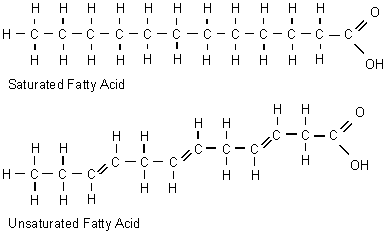
\includegraphics[width=1.0\textwidth]{fas}
\caption[Fatty Acid structure]{The structure of Fatty Acids(FA) which
  consists of a long hydrocarbon side-group. The length of this
  side-group charactersises the FA.}
\label{fig:fas}
\end{figure}

In this study we are interested in the elongation process in its
entirety so our models capture the combined effect of the two pathways
responsible for it, FA biosynthesis \textit{and} FA elongation. In
this section I first introduce the basic model and the assumptions
made to simplify it, the tuning of that basic model based on FA
measurements, a version of the model in stochastic pi-calculus and
finally the extension of the model with the introduction of some
control mechanisms.

\section{Basic model}
\subsection{Petri Net implementation}
FA biosynthesis starts with Acetyl-CoA which is being converted to
Malonyl-CoA. A reaction between Malonyl-CoA and Acetyl-CoA starts off
the first $C_4$ FA product. After that there are successive $C_2$
concatenations to elongate the FA product with each elongation step
, that requires 4 reactions, requiring another Malonyl-CoA(Figure~\ref{fig:fa_synthesis}). The
full pathway from KEGG can be seen in
Figure~\ref{fig:kegg_synthesis}. The elongation pathway located in ER
is similar in nature but the intermediaries are CoAs instead of
ACPs(Figure \ref{fig:kegg_elongation}). 

\begin{figure}[htbp!]
\centering
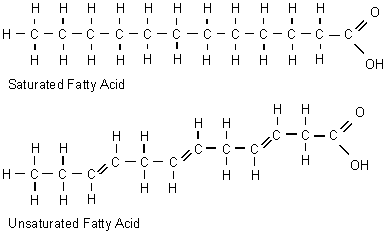
\includegraphics[width=1.0\textwidth]{fas}
\caption[FA structure]{The structure of Fatty Acids(FA) which
  consists of a long hydrocarbon side-group. The length of this
  side-group charactersises the FA.}
\label{fig:fas}
\end{figure}

\begin{figure}[htbp!]
\centering
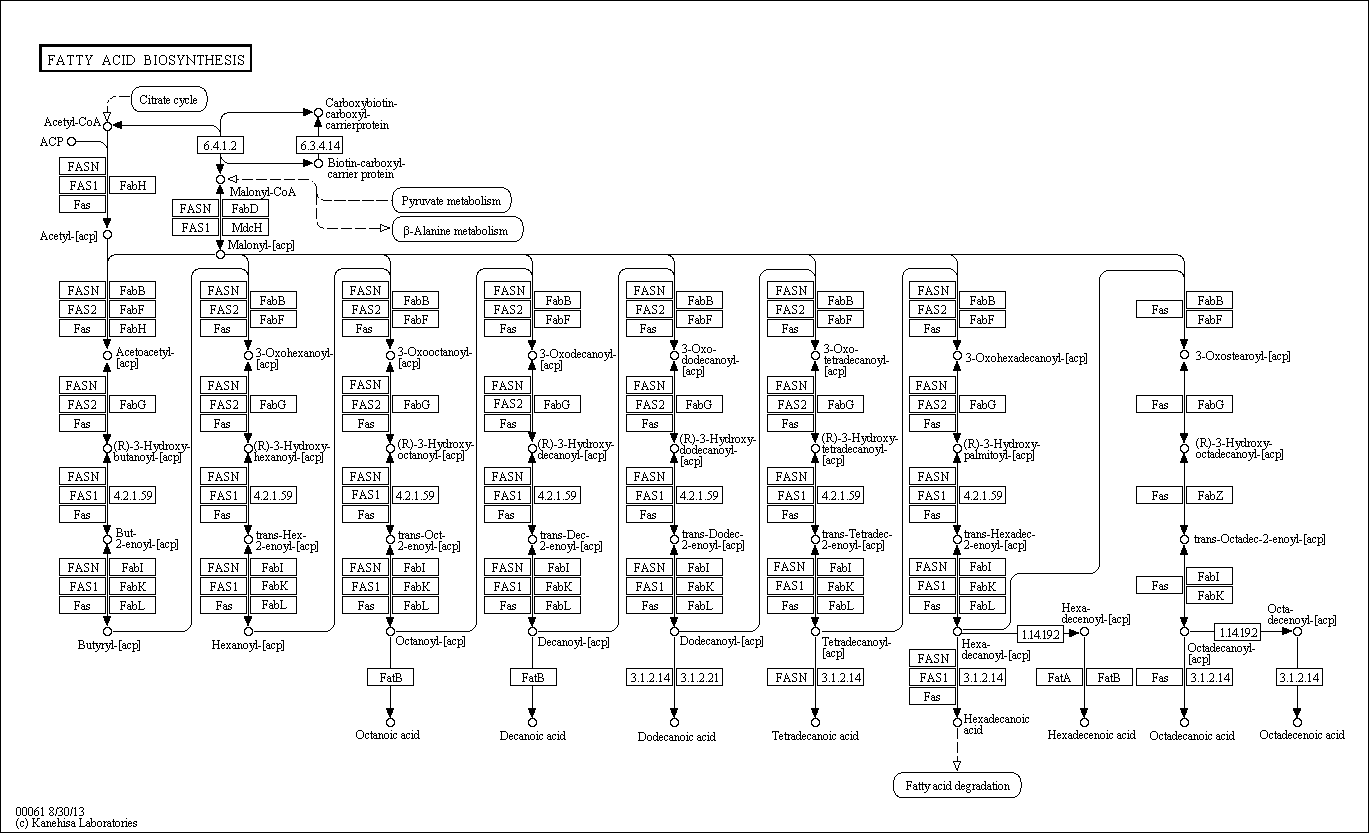
\includegraphics[width=1.0\textwidth]{kegg_synthesis}
\caption[Fatty Acid biosynthsis in cytosol]{FA biosynthesis in the
  cytosol. Notice the successive concatenations. Each concatenation
  takes 4 reactions.}
\label{fig:kegg_synthesis}
\end{figure}

\begin{figure}[htbp!]
\centering
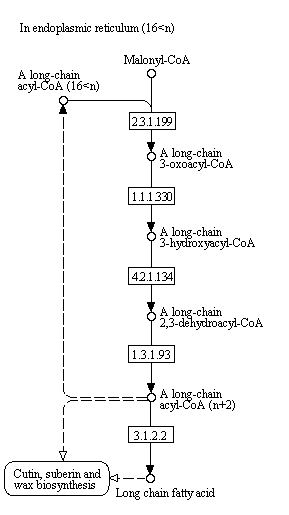
\includegraphics[width=1.0\textwidth]{kegg_elongation}
\caption[Fatty Acid elongation in ER]{General form of FA elongation in
ER. Notice that the intermediate products are CoAs instead of ACPs as
in biosynthesis.}
\label{fig:kegg_elongation}
\end{figure}

Because of the natural correspondence between biochemical reactions as
they are found in the KEGG static model to Petri Net model constructs
a straight translation between the two is straightforward. All the
pathway reactions become transitions with pre-places the reactants and
post-places the products. Here we made our first assumptions by
omitting the enzymes from the reactions. Information about the enzymes
is not so important for our purposes since we are interested in the
numbers of molecules of the metabolites in the system. Information
about the enzymes can be incorporated in the transition rates. 
The net can be animated using its formal
operational semantics and as transitions/reactions occur
tokens/metabolites move through the net. The FA products are
represented as sinks, places that are not pre-places to any
transitions, so once a token reaches one of these sinks it is
trapped. That way the probabilistic iterative nature of the process is
capture completely, an intermediate of the process can either remain
at that length or go on to form longer FAs. The sinks are therefore
the outputs of the stochastic process with the inputs being the places
that do not act as post-places for any transitions. Starting with some
finite number of molecules at the inputs, these will be consumed
throughout the process until we reach a dead-state where no further
transitions are enabled. The translation from the KEGG pathway model
to the Petri Net model was done manually with the SNOOPY \cite []
{heiner2012snoopy}tool which
allows you to draw a net and play the token game for basic nets to
observe its behaviour. 

\begin{figure}[htbp!]
\centering
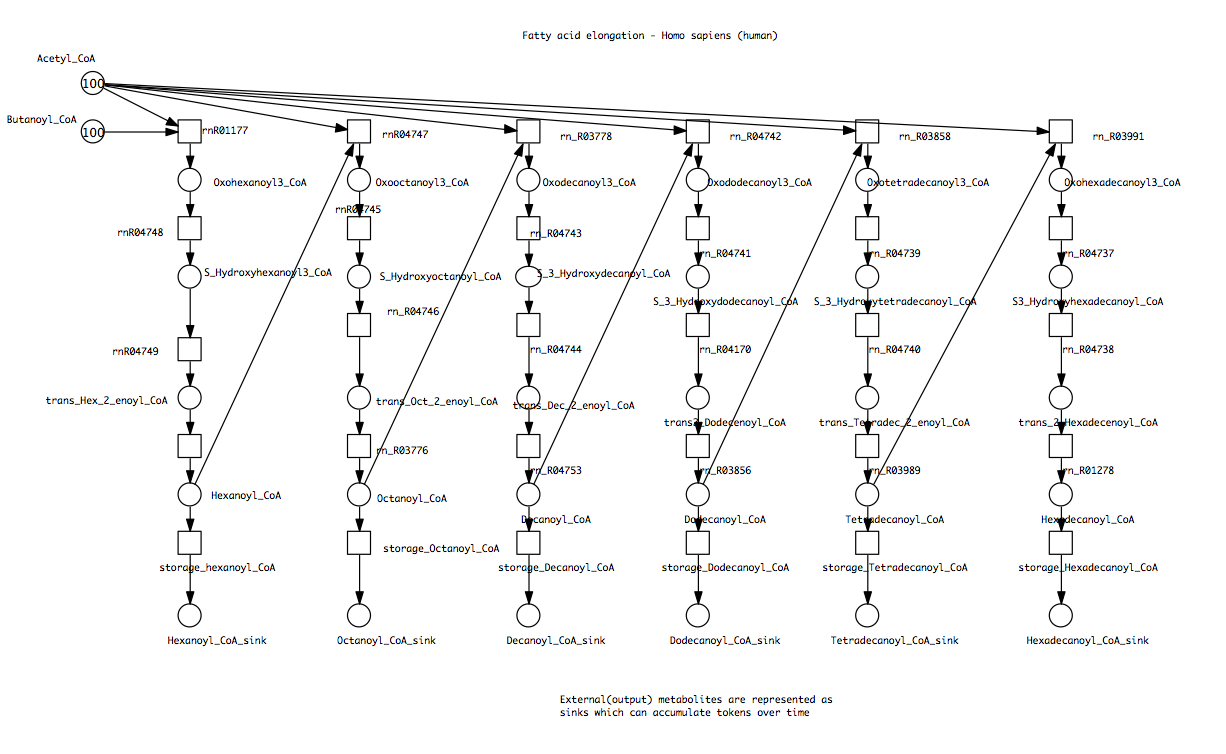
\includegraphics[width=1.0\textwidth]{pn_fa_elongation}
\caption[FA elongation Petri Net model]{}
\label{fig:pn_fa_elongation}
\end{figure}

A direct translation from KEGG is certainly useful for capturing a
low-level biochemical view of the system. The model can offer an even
more fine-control view of the system than the model presented in
Figure~\ref{fig:pn_fa_elongation} by including the enzymes in the
reactions and information about their affinity to the reaction
substrates. However including too many details in the model can
sometimes hide the true aspect of the system the modeller is trying to
understand and analyse. Here we are interested in the probabilistic,
non-deterministic nature of the iterative FA elongation process which
happens as this series of $C_2$ concatenation steps in FA elongation
and biosynthesis pathways in ER and cytosol respectively. The outputs
we are particularly interested to see are the numbers and proportions of FAs at
different lengths. In Petri Nets model language these are the number
and more importantly the proportions
of molecules/tokens that end up in the sink places at the stop of the model
execution. Because the process is inherently iterative and
probabilistic these numbers will be different at the end of each model
execution. This is in contrast with most dynamic modelling approaches
as we are not interested in the time traces but rather only at the end
result of this stochastic process. We can think of the Petri Net as a
magic box governed by some probabilities(that we can tune) where we
throw some inputs and according to these probabilities some output
will come out at the other end in the form of proportions of FAs at different
lengths. The probabilities are just the control parameters that guide
the operation of the magic box.

Having outlined our modelling goals in the previous section we can now
make some assumptions that will guide our design of the simplified
synthesis/elongation model that will be our basic model throughout
this study. First of all the model will capture the combined effect of
both the pathways. The two pathways are in different compartments of
the cell, one in cytosol and one in ER, but we will ignore the
transportation of FAs from cytosol to ER and we will assume that the
two process are sequential so a $C_{18}$ for example can be elongated
directly to a $C_{20}$ while in reality it would have to first be
transported to the ER. Since we also take this view of the
net model as a control box turning input signal through a series of
steps to an output signal we can safely squeeze the four step reaction chain
needed for each $C_2$ concatenation step to a single step reaction and
at the same time consider only the forward direction
reactions. Also, since we are no longer consider exact chemical
reactions the reactions rate functions will just be constant values
and we will treat those more as probabilities that will govern the
non-deterministic decisions during the execution of the model that
transforms the input signal to output proportions of FAs. Finally I
also decided to stop the elongation process at $C_{22}$ and that the
sinks will only include products $C_{12}$ - $C_{22}$. FAs with lengths
4-10 will be included but no output will be accumulated there. These
decisions are a bit arbitrary but they are ultimately tied with the
output real datasets I had available for tuning the model(see
subsequent sections).

To build the basic model then that follows from the goals and this
assumptions was built manually with SNOOPY \cite [] {heiner2012snoopy}. This basic model that will
be the basis for our work in this study can be seen in
Figure~\ref{fig:fa_elongation_full}. The model is similar in nature to
the more full model presented previously but the concatenation steps
are represented as single transitions and the elongation process goes
up to $C_{22}$ because the elongation process in the ER is also
included. Starting simple I also started from the inputs Malonyl-CoA
and Acetyl-CoA whereas in reality the only precursor of FA
biosynthesis is Acetyl-CoA and the 2 input points of the pathway are
products coming from Acetyl-CoA. The model as presented in
Figure~\ref{fig:fa_elongation_full} starts with inputs: 300
Malonyl-CoA and 100 Acetyl-CoA molecules. The model can then be set in
motion with SNOOPY until it reaches a dead state which basically
corresponds to the point where the system runs out of input
metabolites to 'fuel' any further reactions. The output of the system
is the number of tokens accumulated at each of the sinks or FAs of
different lengths.

Observing the execution pattern of the basic net model we notice an
execution pattern which leads to an elegant view of the system as a
series of binary probabilistic decisions or Bernoulli trials. The way
the inputs of the model are set up, at the start of the model
execution only the initial transition producing the first product $C_4$ is
enabled. If we consider that after this transition fires (since its
the only one enabled) it 
will only fire again after its initial product has reached a sink then
at each point only one token is travelling through the net. This token
goes through an iteration of binary decisions: stay at current length
\textit{or} continue to form a longer
FA. More formally as the token gets
transformed to an intermediate product there are only two transitions
enabled: the transition taking it to the next longer intermediate and
the transition taking to be stored at its current length(Figure~\ref{fig:binary_decision}). Let these
two transitions be $t_1$ and $t_2$ respectively. According to
the operational semantics of Stochatic Petri Nets(see Methods section)
a wait time is sampled for each of the enabled transitions from a
negative exponential distribution with rate the value of the rate
function of the
transition. In this case the rate function of the two transitions are
constants(see assumptions) $\lambda_{t_1}$ and $\lambda_{t_2}$. Since
we know that one of the reactions will fire we can say that the
firing probabilities of the two transitions or the probabilities of
the token's decisions are:

\begin{align*}
P(staying)& =P(t_1) = \frac{\lambda_{t_1}}{\lambda_{t_1} + \lambda_{t_2}}\\
P(continuing) & = P(t_2) = \frac{\lambda_{t_2}}{\lambda_{t_1} + \lambda_{t_2}} = 1 - P(t_1)\\
\end{align*}

In other words this is a Bernoulli trial with probability of success
$p = P(t_1)$. Since we only care about the outputs at the end of the
execution and not the timeframe of the process from start to finish
then only the ratio of these two successive transitions rates is
important and not their absolute numbers. Then the entire journey of a token through the network
from the initial $C_4$ product until it reaches a sink and gets stored
can be thought of a series of Bernoulli
trials(Figure~\ref{fig:trials}). Then the entire stochastic process
can be thought of a sequence of successive realisations of this series
of trials with tokens travelling through the net one
after the other with each one going through the series of decisions
or Bernoulli trials. The initial assumption that only one token
travels through the net at each time can in fact be dropped since the
output of the net only depends on the ratios of the pair of
transitions representing each binary decision. I just chose to have it
because this leads to the nice picture of the successive realisations
of chains of Bernoulli trials which is intuitive for illustration
purposes.
It is also interesting to note how this binary decision
corresponds to a conflict between two events that share pre-conditions
which create non-determinsim through a race condition between the two
depdendent events. This 'conflict' which represents this decision
process is captured inherently in the structure and semantics of Petri
Nets. 

Each realisation of the stochastic process described by the Petri Net
model which is itself a series of successive realisations of series of
Bernoulli trials will have different outputs. 







\subsection{Model parameters}

\subsubsection{Point estimates}

\subsubsection{Profiles}

\subsection{Execution results}



\section{A stochastic $\pi$-calculus version}





\section{Extended model of FA synthesis}

